\documentclass[10pt]{beamer}
\usecolortheme{spruce}

\usepackage{hyperref}
\usepackage[utf8]{inputenc}
\usepackage[T1]{fontenc}
\usepackage{color}
\usepackage{colortbl}% http://ctan.org/pkg/xcolor
\usepackage{multirow}
\usepackage{textpos}
\usepackage{tcolorbox}
\usepackage{tikz}
\usetikzlibrary{tikzmark,patterns,arrows,shapes,positioning,calc}
\usepackage{tcolorbox}
\usepackage{graphicx}
\usepackage{dsfont}
\usepackage{amsmath}
\usepackage{url}
\usepackage{hyperref}

% slide numbering
\setbeamertemplate{sidebar right}{}
\setbeamertemplate{footline}{%
	\hfill\usebeamertemplate***{navigation symbols}
	\hspace{1cm}\insertframenumber{}/\inserttotalframenumber}

% options
\setbeamerfont{caption}{size=\scriptsize}
\AtBeginSection[] {
	\begin{frame}<beamer>
		\frametitle{Outline}
		\tableofcontents[currentsection]
	\end{frame}
}
\setbeamertemplate{sidebar right}{}
\setbeamertemplate{footline}{%
	\hfill\usebeamertemplate***{navigation symbols}
	\hspace{1cm}\insertframenumber{}/\inserttotalframenumber}

% define title page
\title{Direct and indirect effects of the COVID-19 pandemic on mortality in Switzerland, a population study}
\author{\underline{Julien Riou}$\textsuperscript{1,2}$, Anthony Hauser$\textsuperscript{1,2}$, Anna Fesser$\textsuperscript{2}$, Christian L. Althaus$\textsuperscript{1}$, Matthias Egger$\textsuperscript{2}$, Garyfallos Konstantinoudis$\textsuperscript{3}$}
\institute{$\textsuperscript{1}$ISPM, $\textsuperscript{2}$FOPH, $\textsuperscript{3}$Imperial College}
\date{ 28 September 2022 }



\begin{document}

\frame{\titlepage}

	\frame{
	\frametitle{Disclaimer}
	
	\begin{itemize}
		\item Employed by the \textit{Federal Office of Public Health}
		\item Employed by the \textit{University of Bern}
		\item No conflict of interest
		\bigskip
		\item  Views and opinions expressed belong solely to the author
	\end{itemize}
}

\begin{frame}
\frametitle{Aims}
\begin{enumerate}
	\item Estimate the \alert{excess all-cause mortality} in Switzerland in 2020-2022 by age, canton and epidemic phase (with uncertainty)
	\bigskip
	
	\item Examine the \alert{interplay} between excess mortality and laboratory-confirmed SARS-CoV-2-related deaths

\end{enumerate}
\end{frame}


\begin{frame}
\frametitle{Step 1: estimate the excess all-cause mortality}
Definition: 
\begin{itemize}
 \item excess mortality = observed mortality - expected mortality
 \item counter-factual reasoning: how many deaths would have occurred \alert{had the pandemic not occurred?}
\end{itemize}

\bigskip
Extrapolate from:
\begin{itemize}
	\item historical trends in mortality data (seasonality, yearly trends)
	\item by location, age, sex
	\item account for changes in the population (extrapolate from 2010-2019)
	\item account for key covariates: temperature (ERA5), public holidays
	\item account for geographical structure (BYM structure\footnote{Besag, York \& Mollié (1991)})
%	\item Rerunning Bayesian model previously developed by Konstantinoudis et al.
\end{itemize}
\bigskip
Poisson model fitted in INLA, cross-validated\footnote{Konstantinoudis et al (2022)}
\end{frame}

%\begin{frame}
%\frametitle{Step 1: data}
%
%Demographic data from the \alert{Federal Statistical Office}:
%\begin{itemize}
%	\item 
%
%\end{itemize}
%
%\end{frame}
%
%\begin{frame}
%	\frametitle{Step 1: estimate the expected mortality}
%	Poisson regression\alert{Bayesian spatio-temporal model}\footnote[frame]{ G. Konstantinoudis et al., \textit{Regional excess mortality during the 2020 COVID-19 pandemic in five European countries} (Nature Communications, 2022)}  providing estimates of expected mortality in 2020-2022 from mortality data in 2014-2019:
%	\begin{itemize}
%		\item by week
%		\item by age group (0-39, 40-59, 60-69, 70-79 and 80+)
%		\item by canton
%	\end{itemize}
%	\bigskip
%	
%	Adjusting for:
%	\begin{itemize}
%		\item population trends (extrapolated from data on Dec. 31st 2010-2019)
%		\item temperature
%		\item public holidays
%	\end{itemize}
%\end{frame}


\begin{frame}
	\frametitle{Results: Excess mortality}
	Over the full study period (February 24, 2020 to April 3, 2022):
	\begin{itemize}
	\item \alert{156,193 observed deaths} from all causes in Switzerland 
	\item \alert{142,408} (95\% CrI: 138,044 to 149,125) expected deaths had the pandemic not occurred
	\item \alert{13,786} (95\% CrI: 7,068 to 18,149) excess all-cause deaths 
	\item a relative increase of \alert{9.7\%} (95\%CrI: 4.7 to 13.1)
	\end{itemize}
	\bigskip\bigskip
	NB: this includes all sources of uncertainty (population, effect of covariates)
\end{frame}

\begin{frame}
	\frametitle{Results: Excess mortality}
	Break-down by \alert{epidemic phase}:
	\begin{figure}[t]
		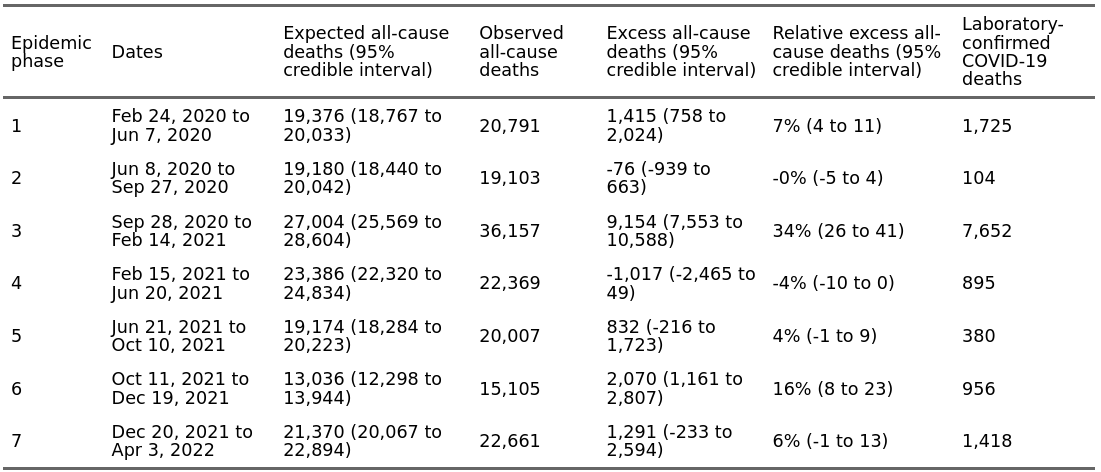
\includegraphics[width=\linewidth ]{figures/table1.png}
		\caption{Number of expected and observed deaths from all causes, estimated excess mortality and laboratory-confirmed COVID-19-related deaths by seven epidemic phases between February 2020 and April 2022.}
	\end{figure}
\end{frame}


\begin{frame}
\frametitle{Results: Excess mortality}
\begin{figure}[t]
	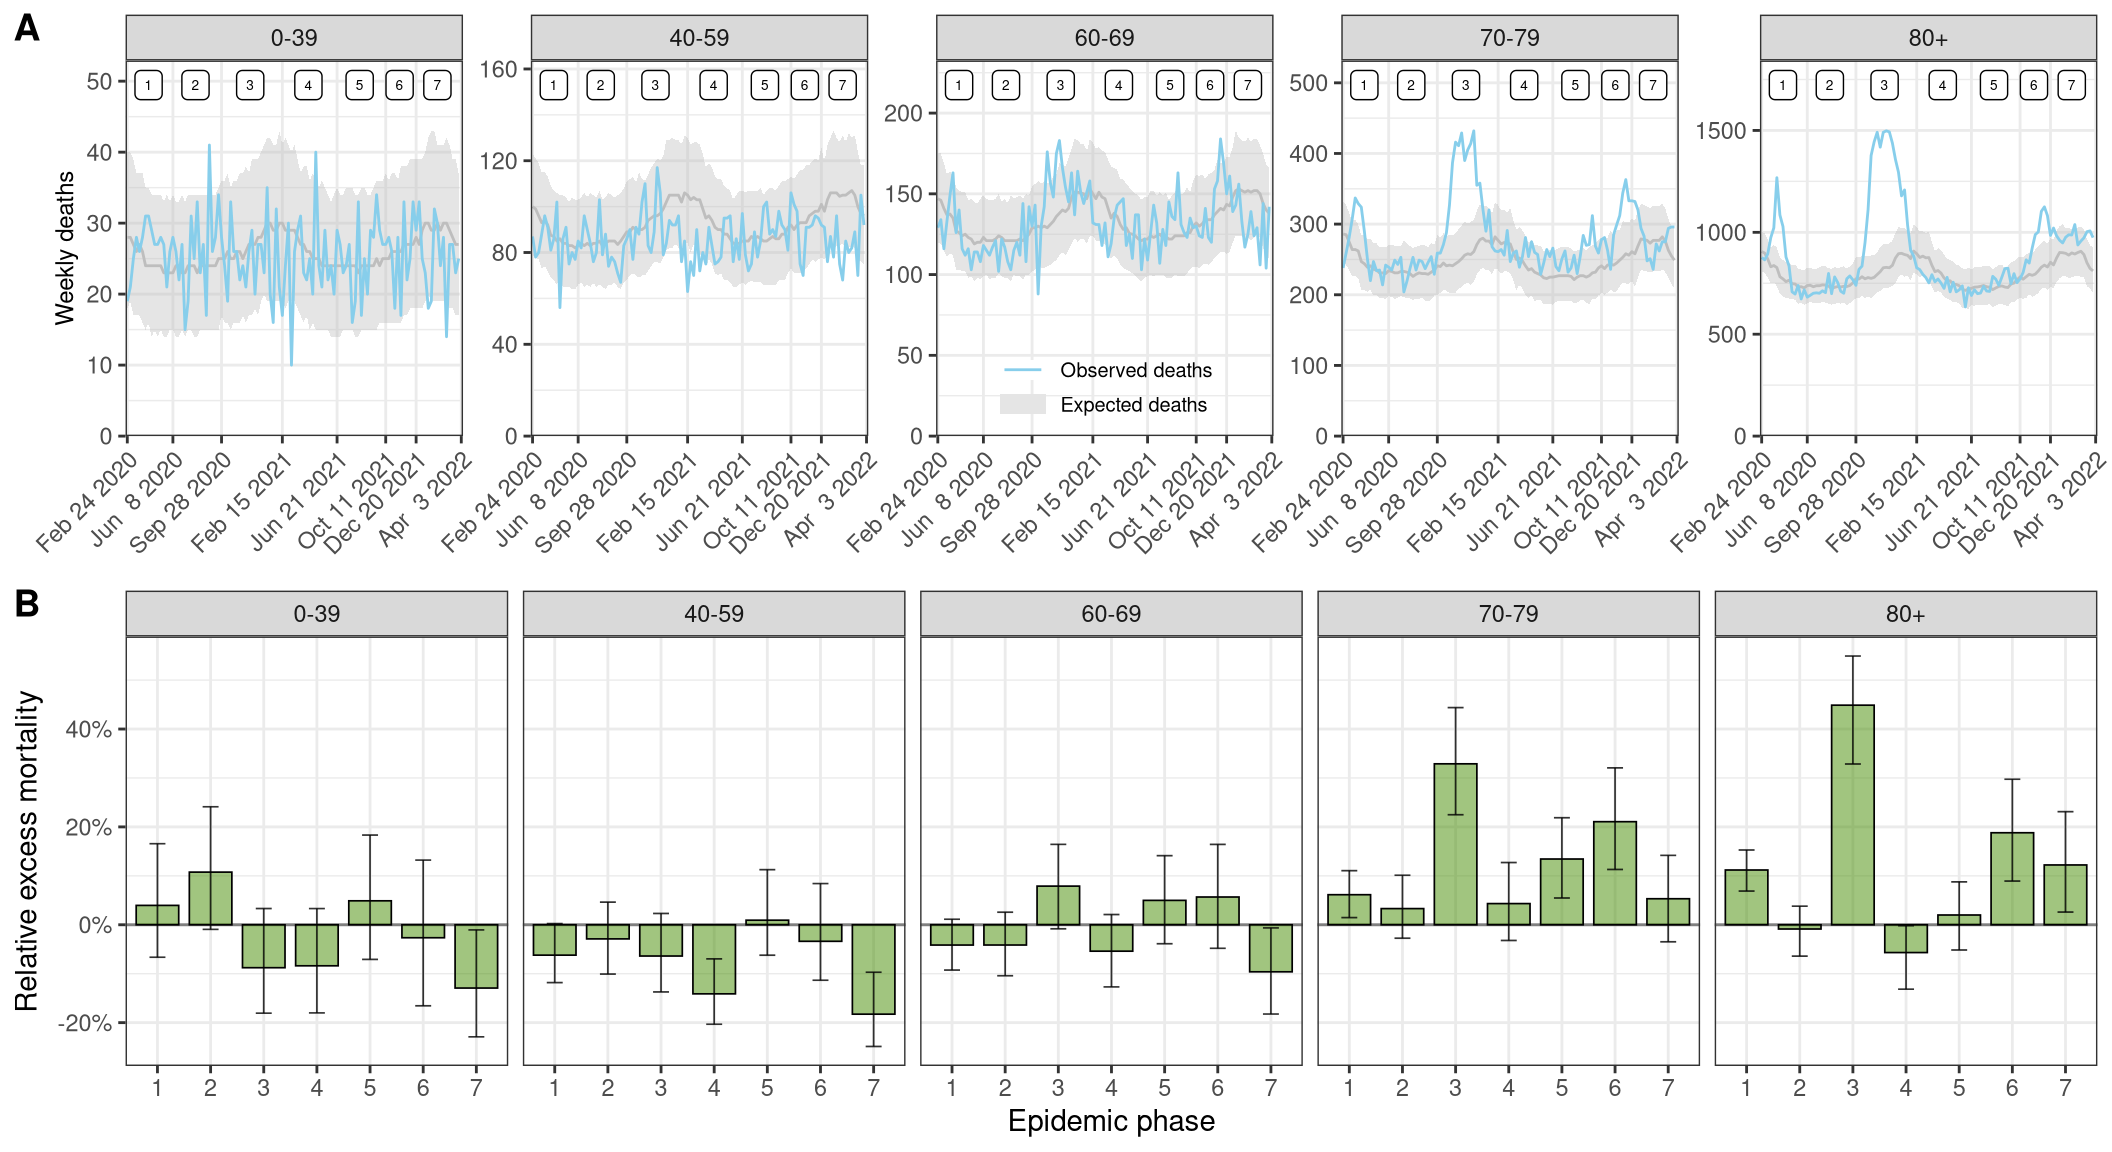
\includegraphics[width=\linewidth ]{figures/fig1.png}
	\caption{(A) Observed and expected number of weekly deaths by age group in Switzerland from February 2020 to April 2022. Model-predicted expected deaths are shown with median and 95\% credibility interval. Numbers at the top indicate epidemic phases 1 to 7. (B) Estimated relative excess mortality by seven epidemic phases from February 2020 to April 2022 and five age groups. Medians with 95\% credible intervals are shown.}
\end{figure}
\end{frame}



\begin{frame}
\frametitle{Step 2: excess mortality vs. SARS-CoV-2 deaths}
\alert{Visual comparison}:
\begin{figure}[t]
	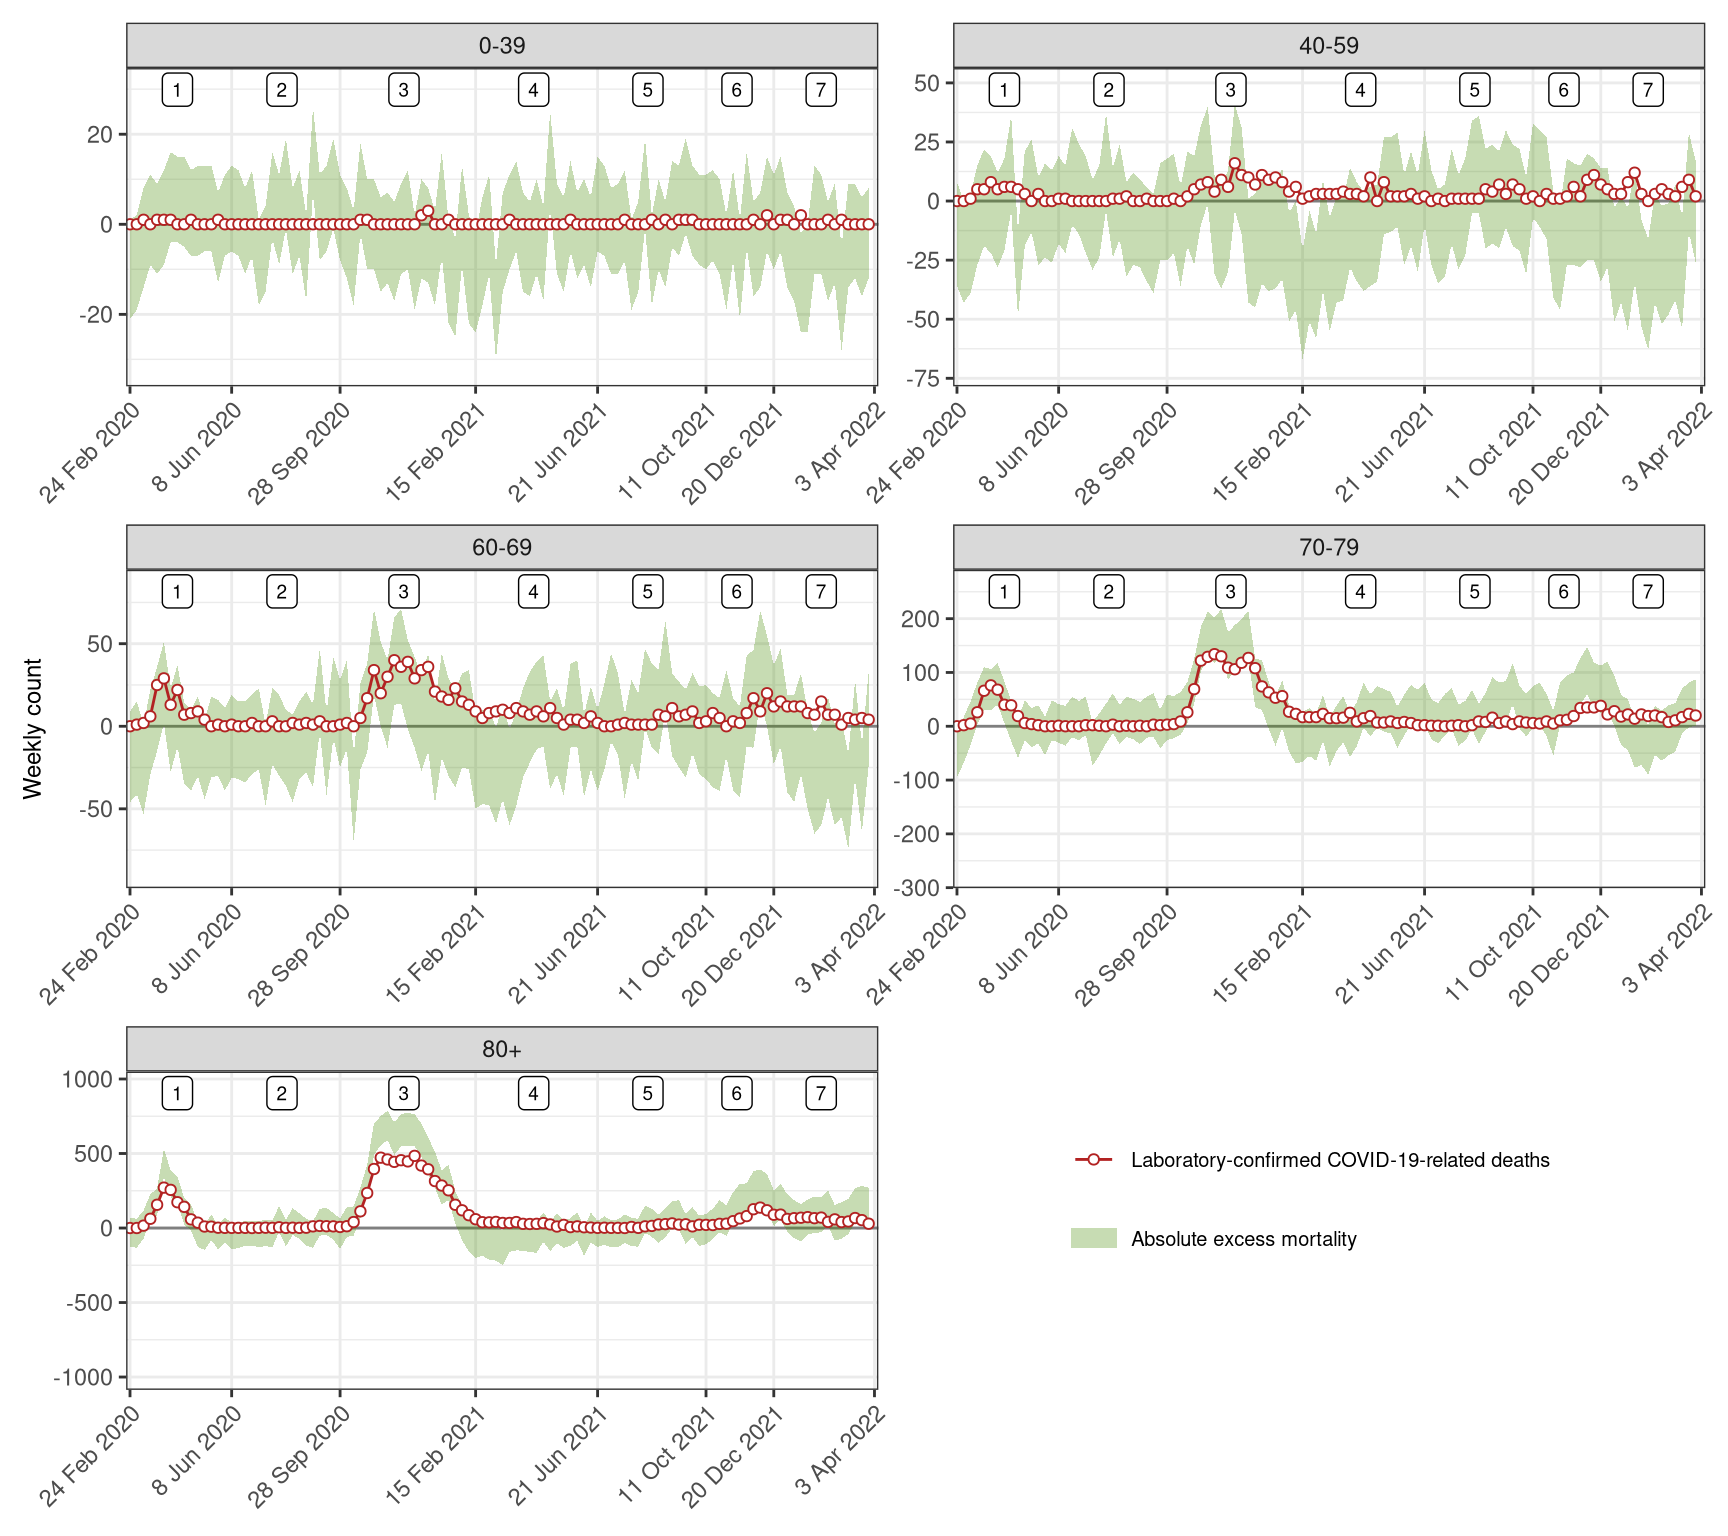
\includegraphics[width=.8\linewidth ]{figures/fig2.png}
	\caption{Excess all-cause deaths and laboratory-confirmed SARS-CoV-2-related deaths in Switzerland in 2020-2021 over time.}
	
\end{figure}
\end{frame}

\begin{frame}
	\frametitle{Step 2: excess mortality vs. SARS-CoV-2 deaths}
	Overall correlation coefficient: \alert{0.89} (95\%CrI: 0.85 to 0.92)
	\begin{figure}[t]
		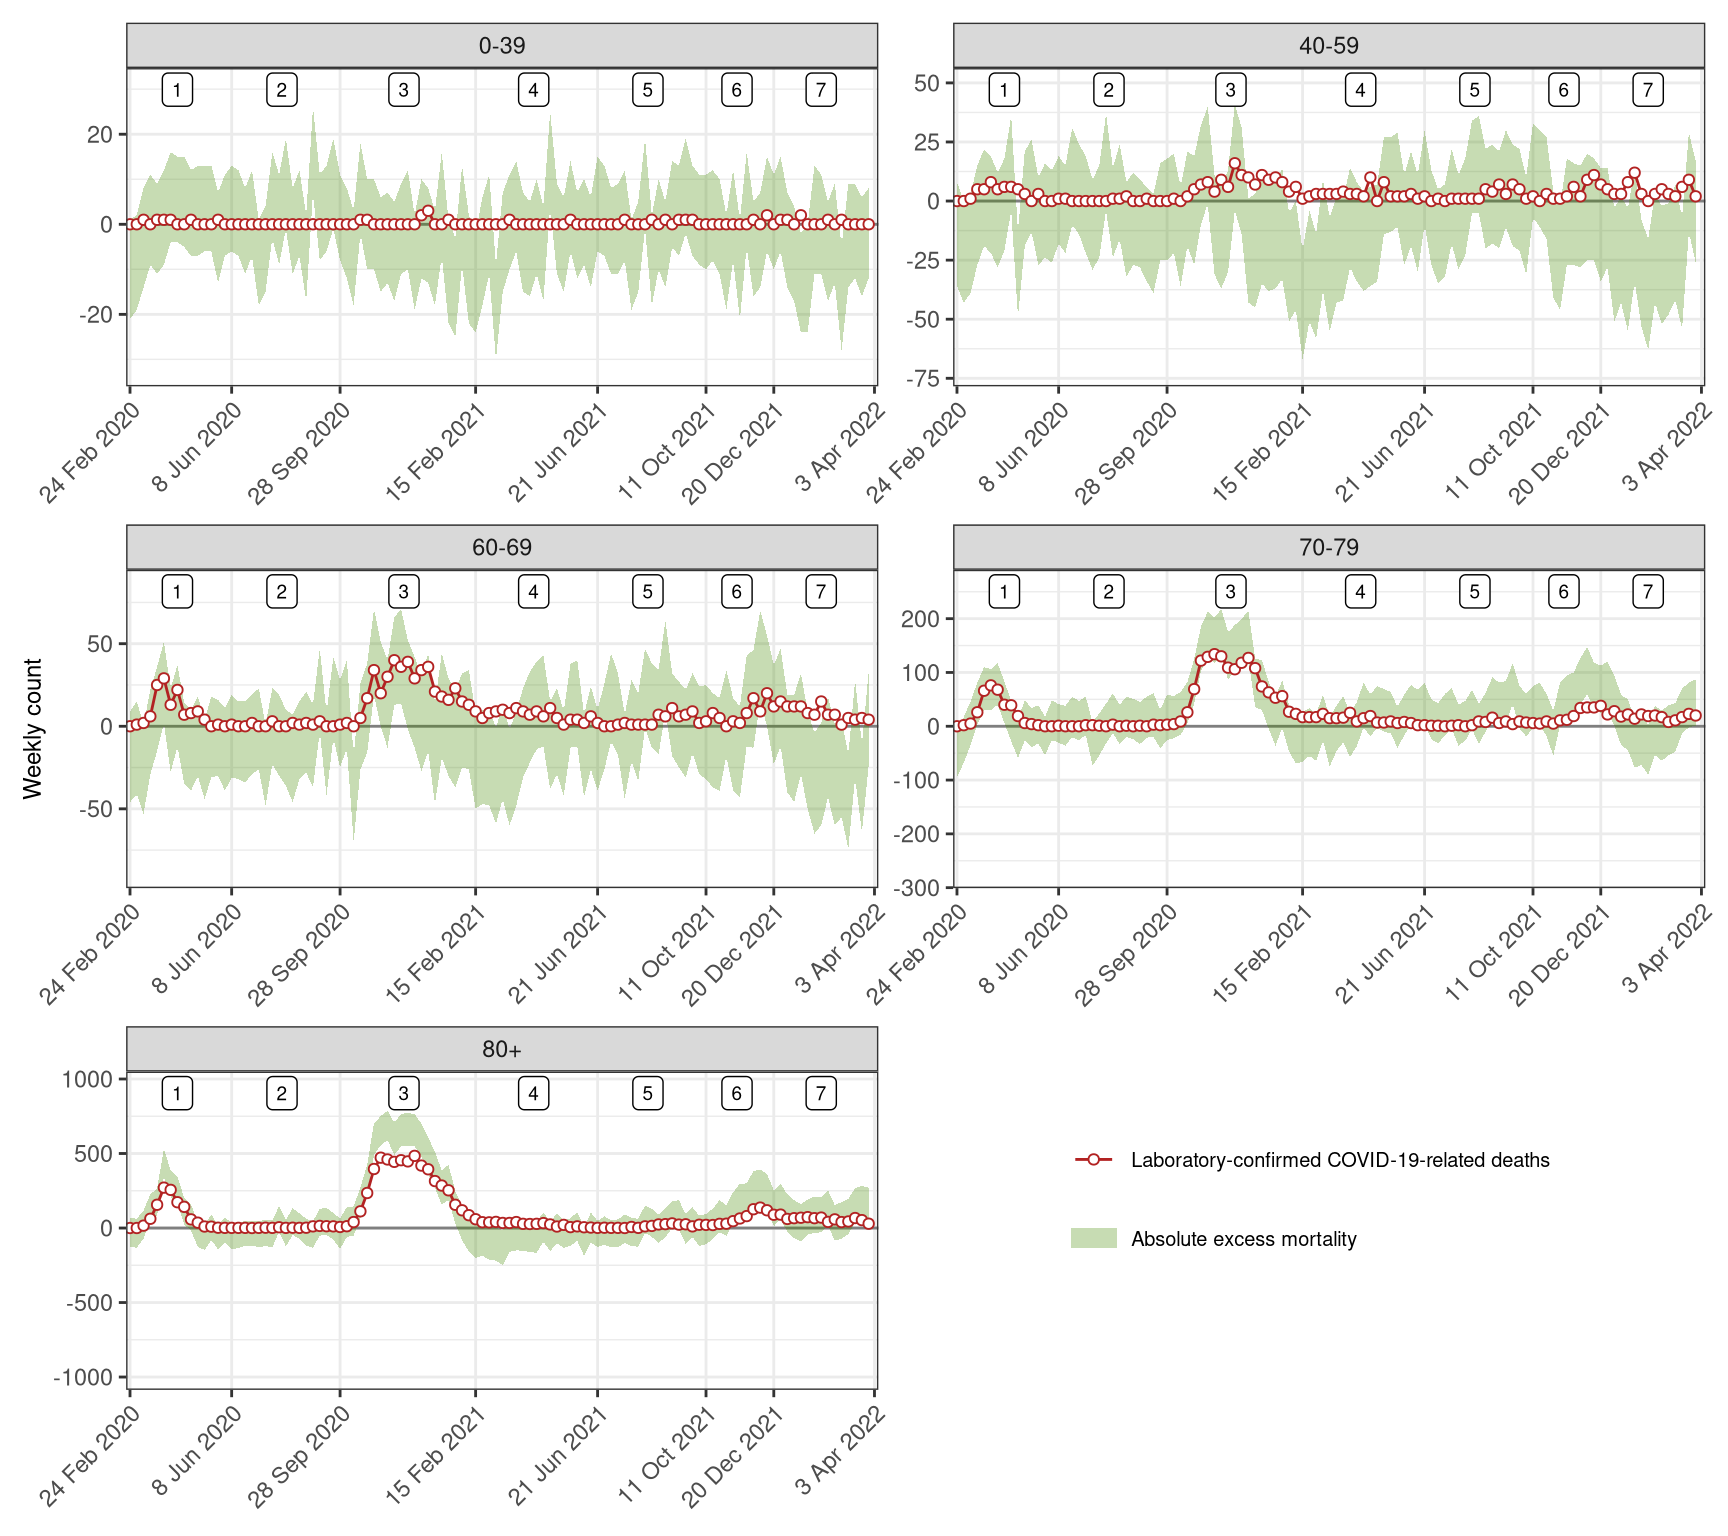
\includegraphics[width=.8\linewidth ]{figures/fig2.png}
		\caption{Excess all-cause deaths and laboratory-confirmed SARS-CoV-2-related deaths in Switzerland in 2020-2021 over time.}
		
	\end{figure}
\end{frame}


\begin{frame}
\frametitle{Step 2: excess mortality vs. SARS-CoV-2 deaths}
\alert{Statistical approach} using modified Poisson regression (no intercept):
$$\text{O}_{t} \sim \text{Poisson}\left( \beta_1\text{L}_{t} + \beta_2\text{E}_{t} \right)$$
where:
\begin{itemize}
\item $\text{O}_{t}$ is the observed number of all-cause deaths on week $t$
\item $\text{L}_{t}$ is the number of laboratory-confirmed SARS-CoV-2 deaths
\item $\text{E}_{t}$ is the expected number of all-cause deaths given historical trends
\end{itemize}
\end{frame}


\begin{frame}
\frametitle{Step 2: excess mortality vs. SARS-CoV-2 deaths}
$$\text{O}_{t} \sim \text{Poisson}\left( \alert{\beta_1\text{L}_{t}} + \beta_2\text{E}_{t} \right)$$
\bigskip

\underline{\smash{Interpretation}}: $\beta_1$ is the additional number of observed deaths \alert{for each unit increase in laboratory-confirmed deaths}, controlling for expected deaths:
	\begin{itemize}
		\item if $\beta_1=1$ $\rightarrow$ perfect ascertainment of SARS-CoV-2 deaths
		\item if $\beta_1>1$ $\rightarrow$ more deaths attributable to SARS-CoV-2 than laboratory-confirmed deaths
	\end{itemize}
\bigskip

\alert{$\Rightarrow$} $\beta_1$ measures the \alert{direct effect} of the pandemic on mortality 
\bigskip

\alert{$\Rightarrow$} $\beta_1 \times \text{L}_{t}$ is the total number of deaths directly attributable to SARS-CoV-2 infections
\bigskip

\alert{$\Rightarrow$} $1/\beta_1$ corresponds to the ascertainment of SARS-CoV-2-related deaths

\end{frame}

\begin{frame}
	\frametitle{Step 2: excess mortality vs. SARS-CoV-2 deaths}
	$$\text{O}_{t} \sim \text{Poisson}\left( \beta_1\text{L}_{t} + \alert{\beta_2\text{E}_{t}} \right)$$
	\bigskip
	
	\underline{\smash{Interpretation}}: $\beta_2$ is the additional number of observed deaths \alert{for each unit increase in the expected number of all-cause deaths}, controlling for SARS-CoV-2 deaths:
	\begin{itemize}
		\item if $\beta_2=1$ $\rightarrow$ as many ``all-cause-except-SARS-CoV-2'' deaths than expected
		\item if $\beta_2<1$ $\rightarrow$ fewer ``all-cause-except-SARS-CoV-2'' deaths than expected
	\end{itemize}
	\bigskip
	
	\alert{$\Rightarrow$} $\beta_2$ measures the \alert{indirect effect} of the pandemic on mortality
	
\end{frame}

%

\begin{frame}
	\frametitle{Results: direct effect}
	Overall $\beta_1$ is estimated to \alert{1.38 (1.22 to 1.54)}:
	\begin{itemize}
		\item \alert{22\% to 54\% more deaths} directly attributable to SARS-CoV-2 than confirmed over the whole period
		\item or equivalently an \alert{ascertainment of 65\% to 82\%} ($1/\beta_1$) of deaths directly attributable to SARS-CoV-2
		\item given 13,130 laboratory-confirmed deaths, this implies \alert{16,000 to 20,000 COVID-19 deaths} directly attributable to COVID-19 in Switzerland over the period
	\end{itemize}
\end{frame}

\begin{frame}
	\frametitle{Results: indirect effect}
	After \alert{accounting for deaths directly attributable to COVID-19}, the observed number of all-cause deaths was slightly \alert{lower than expected}
	\begin{itemize}
		\item $\beta_2$ estimated to 0.97 (0.93 to 1.01)
		\item 3\% (-1 to 7) fewer all-cause deaths than expected (after accounting for...)
		\item corresponding to 4,406 (-1,776 to 10,700) fewer deaths overall
	\end{itemize}
\end{frame}

\begin{frame}
	\frametitle{Results: variations}
	Variations of $\beta_1$ by age and epidemic phase:
	\begin{figure}[t]
		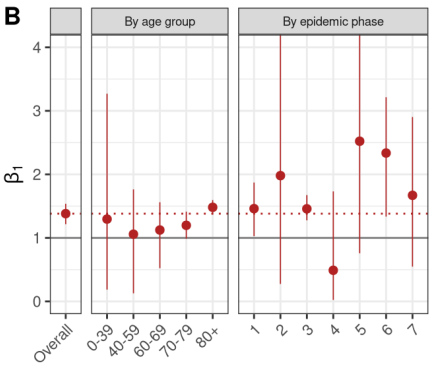
\includegraphics[width=.45\linewidth ]{figures/fig3b.png}
		\caption{Estimates of $\beta_1$, the additional number of deaths to be observed for each unit increase in laboratory-confirmed deaths, after adjusting for the expected number of all-causes deaths given historical trends.}
	\end{figure}
	\begin{itemize}
	\item more deaths were not ascertained in \alert{age groups 70-79 and 80+}
	\item lower ascertainment during phases 1, 3 and 6 (\alert{large epidemic waves})
\end{itemize}
\end{frame}

\begin{frame}
	\frametitle{Results: variations}
	Variations of  $\beta_2$  by age and epidemic phase:
	\begin{figure}[t]
		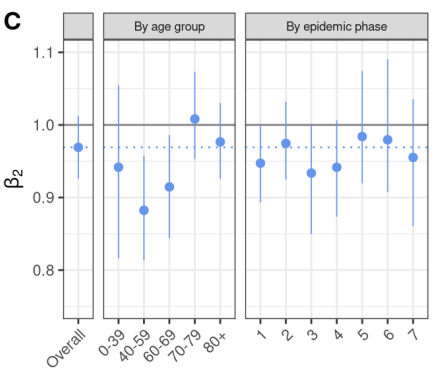
\includegraphics[width=.45\linewidth ]{figures/fig3c.png}
	\caption{ Estimates of $\beta_2$, the additional number of deaths to be observed for each unit increase in the expected number of all-cause deaths, after adjusting for the direct effect of SARS-CoV-2 infections. Estimates of  and  are shown for the whole period, by phase and by age group.}

	\end{figure}
	\begin{itemize}
		\item deficit in all-cause deaths more pronounced in \alert{age groups 40 to 69}
		\item and during phases 1, 3 and 4 (more stringent control measures)
	\end{itemize}
\end{frame}


\begin{frame}
\frametitle{Conclusions}
Summary of results and interpretations:
\begin{itemize}
	\item estimates of excess generally in line with other studies (except WHO)
	\item \alert{1.2-1.5 times more deaths directly caused by COVID-19} than the number of laboratory-confirmed deaths (or reciprocally only 70\% of deaths were ascertained)
	\begin{itemize}
		\item[-] compatible with recent multi-country study (1.29)\footnote{Wang et al (2022)}
		\item[-] cause of deaths 2020: 24-33\% more COVID-19 deaths than FOPH
		\item[-] lower ascertainment during periods of high epidemic activity
		\item[-]concentrated in older age groups, pointing towards nursing homes\footnote{Li et al (2020)}
	\end{itemize}
	\item \alert{3\% (-1 to 7) fewer all-cause deaths than expected} (after accounting for deaths directly caused by COVID-19)
	\begin{itemize}
		\item[-] concentrated in age groups 40 to 69 and phases 1, 3, 4
		\item[-] protective effect of control measures rather than harvesting/influenza
		\item[-] mechanism unknown (lower pollution, traffic, contacts, activities...)
		\item[-] no argument towards overall harmful effect (does not refute harmful effects from control measures e.g. delays in care, suicide, substance use, violence...)
	\end{itemize}
\end{itemize} 
\end{frame}

\begin{frame}
	\frametitle{Conclusions}
Strengths and limitations:
\begin{itemize}
	\item[+] statistically rigorous approach
	\item[+] accounts for projected population sizes and temperature
	\item[+] full uncertainty propagation
	\item[-] all deaths with a positive test considered caused by COVID-19
	\item[-] ecological bias
	\item[-] assumptions about population changes and mortality in 2020-2022 had the pandemic not occurred
\end{itemize}
\end{frame}


\end{document}